\chapter{Korišteni modeli strojnog učenja}
\label{ch:koristeni-modeli-strojnog-ucenja}
U svrhu raspoznavanja rukom pisanih znakova u ovom radu razmatrane su određene tehnike i modeli strojnog učenja. Ovo
poglavlje detaljno opisuje korišten model neuronske mreže kao i algoritam \emph{Backpropagation} koji je korišten za
pronalaženje optimalnih težina neuronske mreže. Točna struktura korištene mreže opisana je
u\ \ref{ch:rezultati-i-analiza}. poglavlju, dok je opis implementacije neuronske mreže i gradijentnog spusta u
programskom jeziku \emph{Scala} opisan u
dodatku\ \ref{ch:implementacija-neuronske-mreze-i-gradijentnog-spusta-u-programskom-jeziku-scala}.


\section{Neuronska mreža}
\label{sec:neuronska-mreza}
Ideja umjetnih neurona javlja se 1943. godine u radu ``A Logical Calculus of Ideas Immanent in Nervous Activity'' u
kojem su Warren McCulloch i Walter Pitts pokazali da je moguće računati logičke funkcije \emph{I}, \emph{ILI} i
\emph{NE} koristeći model umjetnog neurona\footnote{Također poznat kao \emph{TLU} perceptron.}. Pošto se iz navedenih
logičkih funkcija može izgraditi bilo koja \emph{Booleova} funkcija, od umjetnih neurona moguće je izgraditi mrežu koja
predstavlja željenu \emph{Booleovu} funkciju. Međutim, u tom slučaju umjetna neuronska mreža gradi se ručno a ne
učenjem. Suvremeni model neuronske mreže koji se može učiti zasnovan je na ideji bioloških neurona u mozgu. Inspiracija
za ovakav model neuronske mreže javlja se 1949. godine, kada Britanski biolog Donald Hebb objavljuje knjigu
``The Organization of Behavior'' u kojoj iznosi svoje spoznaje o radu i interakciji bioloških neurona. Glavna spoznaja
bila je ta da ako dva neurona često zajedno pale, tada dolazi do metaboličkih promjena koje uzrokuju povećanje
efikasnosti kojom jedan neuron pobuđuje drugoga. To zapažanje bilo je preduvjet za definiranje algoritma učenja
\emph{TLU} perceptrona kojeg je opisao Frank Rosenblatt u izvještaju
``The Perceptron: A Perceiving and Recognizing Automaton'' iz 1957. godine, te u knjizi ``Principles of Neurodynamics''
iz 1962. godine\ \citep{cupic2013}.

\subsection{Model neurona}
\label{subsec:model-neurona}
Sastavni dio neuronske mreže je pojedinačni neuron. Skup neurona čini jedan sloj neuronske mreže dok se međusobnim
povezivanjem slojeva dobiva umjetna neuronska mreža željene strukture. Jedan neuron može se definirati kao skalarna
funkcija određenog broja ulaza. Neuron se sastoji od ulaza $x_1$ do $x_n$, težina $w_1$ do $w_n$, pobude $net$ te
prijenosne funkcije $f(net)$ koja daje izlaznu vrijednost neurona\ \citep{cupic2013}. Uz težine $w_1$ do $w_n$ još se
obično nalazi težina $w_0$ koja predstavlja prag paljenja neurona. Ukupna pobuda $net$ računa se na sljedeći način:\\
\begin{equation*}
    net = w_0 + \sum_{i = 1}^{n} w_i \cdot x_i.
\end{equation*}
\\
\begin{figure}[htb]
    \centering
    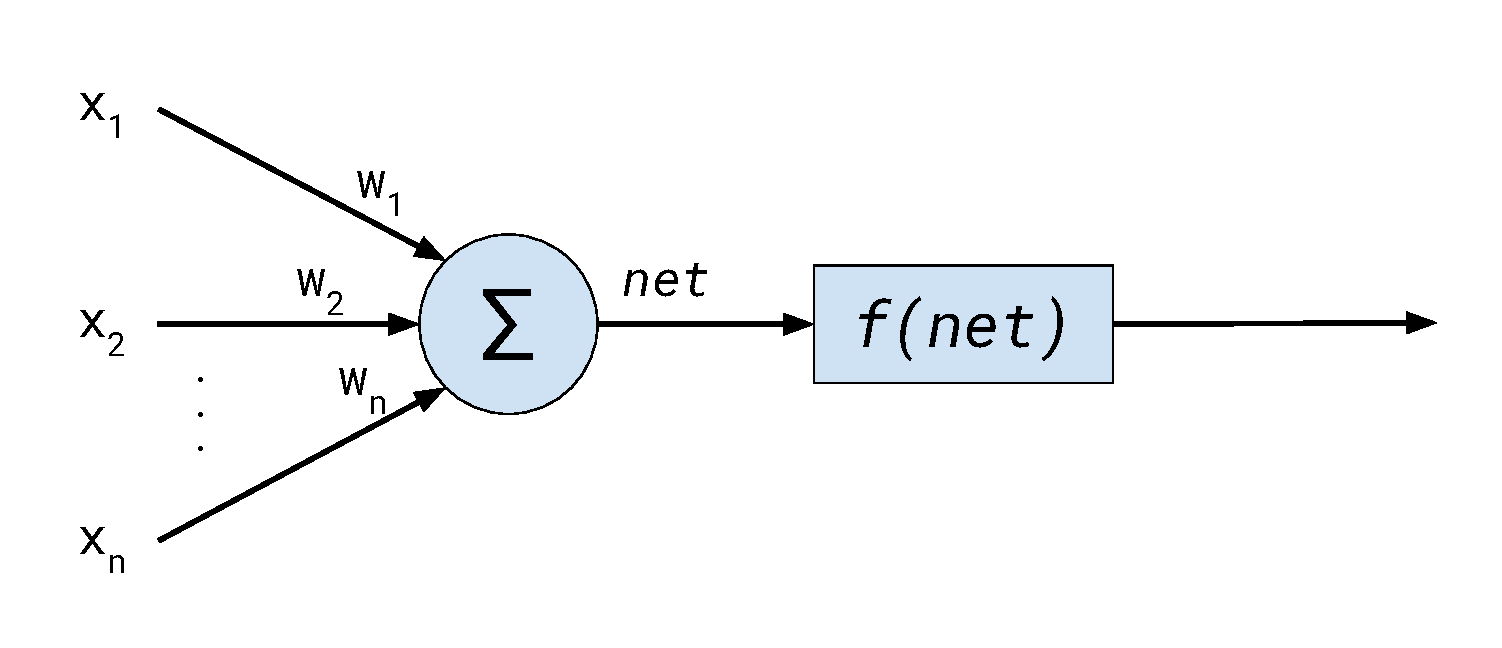
\includegraphics[width=12cm]{images/chapter3/artificial-neuron-model.pdf}
    \caption{Model umjetnog neurona.}
    \label{fig:model-umjetnog-neurona}
\end{figure}
Izlaz neurona računa se kao: $y = f(net)$ gdje je $f$ neka prijenosna funkcija. U ovom radu korištena je isključivo
logistička\footnote{Također poznata kao sigmoida.} prijenosna funkcija koje je prikazana na
slici\ \ref{fig:logistic-function} te je definirana na sljedeći način:\\
\begin{equation*}
    f(x) = \frac{1}{1 + e^{-x}}.
\end{equation*}
\\
Ovakva prijenosna funkcija je veoma praktična jer je njena izlazna vrijednost ograničena na raspon $[0, 1]$ pa njen
izlaz možemo protumačiti kao vjerojatnosnu vrijednost. Logistička funkcija je također derivabilna i njena derivacija
glasi:\\
\begin{equation}
    \frac{df(x)}{dx} = f(x) \cdot (1 - f(x)). \label{eq:logistic-derivation}
\end{equation}\\
Ova derivacija koristit će se u izvodima u odjeljku\ \ref{sec:algoritam-backpropagation}.
\begin{figure}[htb]
    \centering
    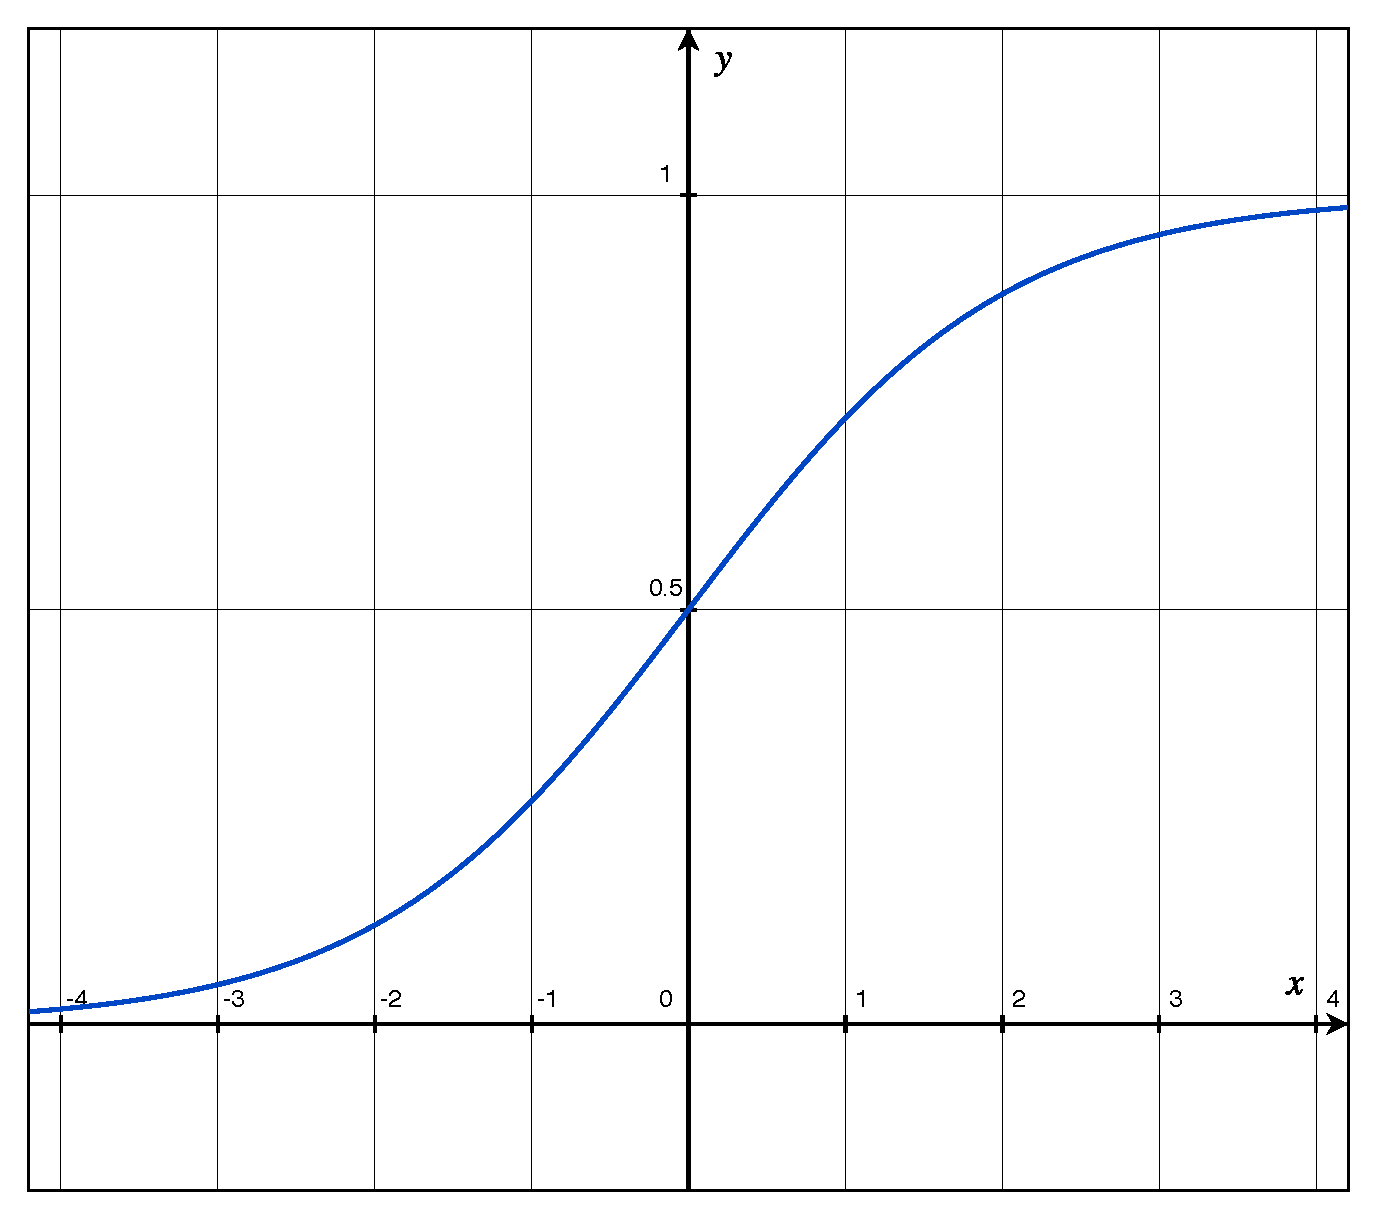
\includegraphics[width=10cm]{images/chapter3/logistic-function.pdf}
    \caption{Graf logističke prijenosne funkcije.}
    \label{fig:logistic-function}
\end{figure}
Ideja navedene strukture neurona dolazi od bioloških neurona koji se sastoje od dendrita, tijela neurona i
aksona. Biološki neuron prikuplja električne impulse preko dendrita koje akumulira u tijelu. Kada se nakupi određena
količina naboja, neuron akumulirani naboj šalje kroz svoj akson prema drugim neuronima\ \citep{cupic2013}. Analogno
tome, kod modela umjetnog neurona dendrite predstavljaju ulazi $x_1$ do $x_n$, pobuda $net$ predstavlja tijelo neurona
dok prijenosna funkcija $f(net)$ predstavlja akson. Slika\footnote{Slika je preuzeta i prilagođena
iz\ \citep{cupic2013}.}\ \ref{fig:model-umjetnog-neurona} prikazuje opisani model umjetnog neurona.

\subsection{Unaprijedna neuronska mreža}
\label{subsec:unaprijedna-neuronska-mreza}
Pojedinačni umjetni neuron zasebno može obrađivati samo manje količine podataka. Stoga više neurona povezujemo u
mrežu u kojoj neuroni mogu biti međusobno povezani u različite strukture. S obzirom na strukturu, umjetne neuronske
mreže dijele se na\ \citep{cupic2013}:
\begin{enumerate}
    \item Unaprijedne mreže: linearne mreže, višeslojni perceptron te mreže s radijalnim baznim funkcijama.
    \item Mreže s povratnim vezama: \emph{Boltzmannov} stroj, mreže s vremenskim pomakom.
\end{enumerate}
U ovom radu korištena je isključivo slojevita neuronska mreža, također poznata kao višeslojni
perceptron\footnote{Višeslojni perceptron je slojevita neuronska mreža koja koristi logističku prijenosnu funkciju.}.
Glavno ograničenje ovakve mreže je da određeni sloj mreže može kao ulaz dobiti samo vrijednost izlaza nekog od
prethodnih slojeva mreže. Time će ukupan izlaz mreže ovisiti samo o ulazima mreže\footnote{Za bilo koje fiksne
vrijednosti težinskih parametara $w_n$.} i bit će vremenski stabilan. Tako definirana mreža ima manji kapacitet učenja
nego mreže koje dozvoljavaju povratne veze, međutim glavna prednost ovog pristupa je olakšan način učenja. Ako je
prijenosna funkcija korištena u neuronima mreže derivabilna, tada će i cijela funkcija neuronske mreže biti derivabilna,
što otvara mogućnost učenja mreže gradijentnim spustom koji je opisan u odjeljku\ \ref{sec:algoritam-backpropagation}.
Struktura jednostavne unaprijedne neuronske mreže prikazana je na slici\footnote{Slika je preuzeta i prilagođena
iz\ \citep{cupic2013}.}\ \ref{fig:simple-neural-network}.
\begin{figure}[htb]
    \centering
    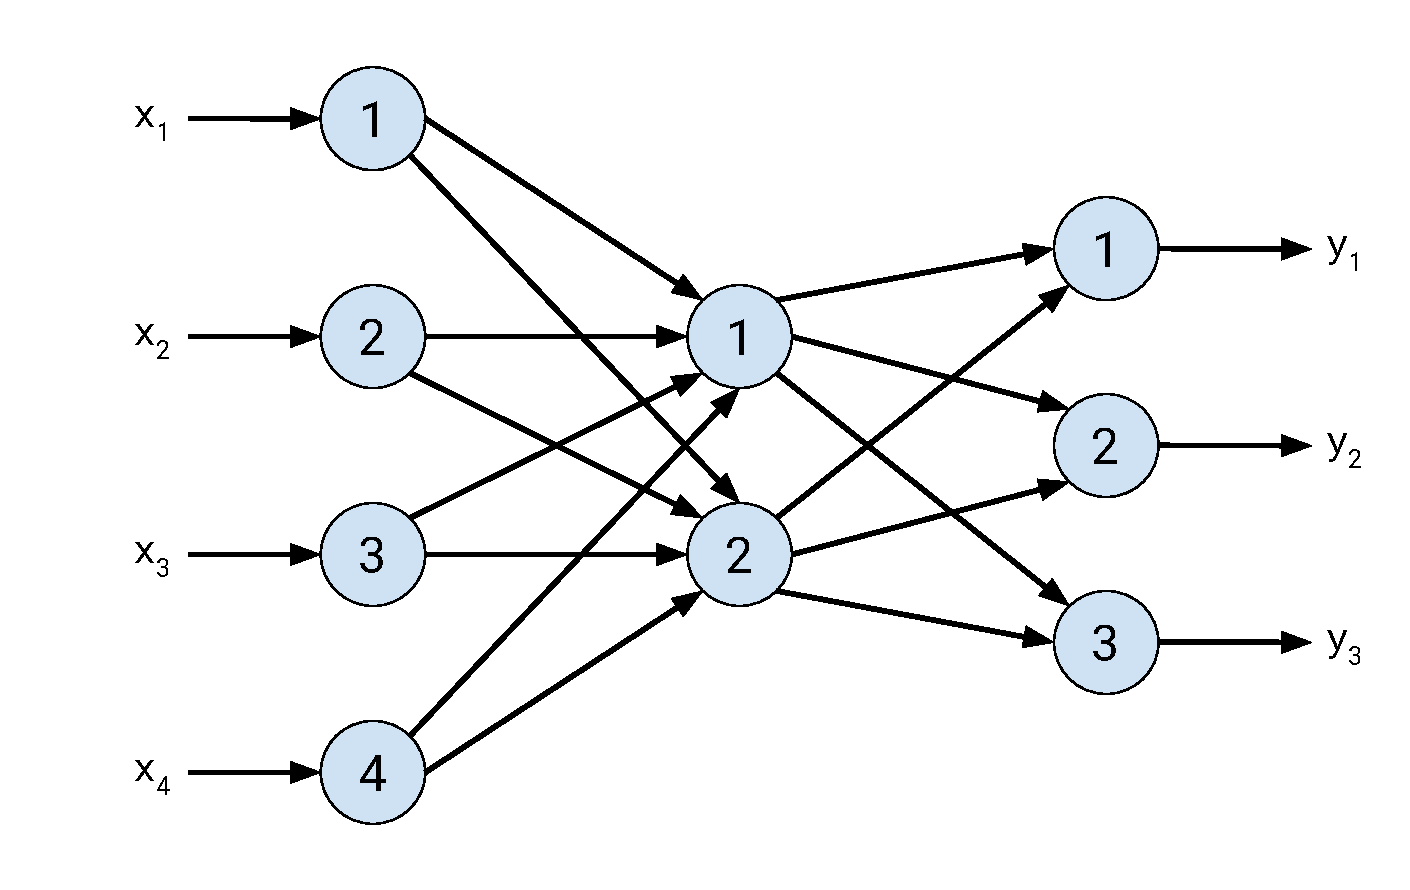
\includegraphics[width=12cm]{images/chapter3/simple-neural-network.pdf}
    \caption{Struktura jednostavne unaprijedne neuronske mreže.}
    \label{fig:simple-neural-network}
\end{figure}
Prikazana neuronska mreža sastoji se od tri sloja:
\begin{enumerate}
    \item sloj koji se sastoji od neurona koji ne obavljaju nikakvu obradu podataka već samo preslikavaju dobivene
    ulazne vrijednosti na svoj izlaz te ih tako čine dostupnima ostatku mreže. Stoga je ovaj sloj ulazni sloj mreže i
    mreža ima 4 ulazna.
    \item sloj čini skriveni sloj mreže koji svoje dobiva ulaze od prvog sloja mreže te svoje izlaze šalje trećem sloju
    mreže.
    \item sloj je izlazni sloj mreže. Ulazne vrijednosti su isključivo vrijednosti izlaza drugog sloja mreže. Pošto ovaj
    sloj ima 3 neurona, cijela mreža će imati 3 izlazne vrijednosti. Time se struktura umjetne neuronske mreže na
    slici\ \ref{fig:simple-neural-network} može definirati kao $4 \times 2 \times 3$.
\end{enumerate}
Struktura neuronske mreže koja je korištena u ovom radu analogna opisanom primjeru, ali s više slojeva većih dimenzija.


\section{Algoritam \emph{Backpropagation}}
\label{sec:algoritam-backpropagation}
Ideja algoritma \emph{Backpropagation} je da se težine neuronske mreže mogu pronaći koristeći gradijentni spust. To se
postiže tako da se težine neuronske mreže korigiraju u svakom koraku algoritma koristeći vrijednost derivacije funkcije
greške mreže. Kako bi to bilo moguće, funkcija greške kao i funkcija koju opisuje neuronska mreže moraju biti
derivabilne. Ovo će biti slučaj kod unaprijednih neuronskih mreža koje koriste derivabilnu prijenosnu funkciju u svim
svojim neuronima, dok kao funkciju greške također možemo odabrati neku derivabilnu funkciju. Za neku unaprijednu
neuronsku mrežu ulazne dimenzije $I$, izlazne dimenzije $O$, $k$ skrivenih slojeva, i izlaznog sloja $k + 1$,
izvod\footnote{Svi izvodi su preuzeti iz\ \citep{cupic2013}.} derivacije započinjemo definiranjem funkcije greške:\\
\begin{equation*}
    E = \frac{1}{2N} \sum_{n = 1}^{N} \sum_{o = 1}^{O} \left(t_{n, o} - y_{n, o}^{(k + 1)}\right)^2
\end{equation*}
\\
gdje $N$ označava broj ulaznih primjera za učenje koji su vektori dimenzije $I$, $t_{n, o}$ je željena vrijednost
$o$-tog izlaza mreže za $n$-ti primjer te je $y_{n, o}^{k + 1}$ vrijednost $o$-tog izlaza mreže za $n$-ti ulazni
primjer. Kako bismo dobili vrijednost korekcije za neku težinu $w_{i, j}^{(k)}$ potrebno je izračunati parcijalnu
derivaciju:\\
\begin{equation*}
    \frac{\partial E}{\partial w_{i, j}^{(k)}}.
\end{equation*}
\\
Tada se težina $w_{i, j}^{(k)}$ korigira na sljedeći način:\\
\begin{equation*}
    w_{i, j}^{(k)} \leftarrow w_{i, j}^{(k)} - \psi \frac{\partial E}{\partial w_{i, j}^{(k)}}
\end{equation*}
\\
gdje je $\psi$ neka mala pozitivna konstanta\footnote{Vrijednost ove konstante znatno utječe na postupak učenja - ako je
njena vrijednost premala, postupak učenja će napredovati jako sporo. S druge strane, prevelika vrijednost uzrokovat će
divergenciju zbog koje će postupak učenja povećavati grešku mreže sve većom brzinom.}.

\subsection{Računanje vrijednosti korekcije težinskih faktora za izlazni sloj neuronske mreže}
\label{subsec:racunanje-vrijednosti-korekcije-tezinskih-faktora-za-izlazni-sloj-neuronske-mreze}
Vrijednost izlaznog sloja $k + 1$ direktno se koristi u izračunu funkcije greške. Stoga parcijalne derivacije težinskih
faktora za izlazni sloj neuronske mreže računamo na sljedeći način:\\
\begin{align*}
    \frac{\partial E}{\partial w_{i, j}^{(k)}} & = \frac{\partial}{\partial w_{i, j}^{(k)}} \left[\frac{1}{2N}
    \sum_{n = 1}^{N} \sum_{o = 1}^{O} \left(t_{n, o} - y_{n, o}^{(k + 1)}\right)^2\right]\\
    & = \frac{1}{2N} \sum_{n = 1}^{N} \sum_{o = 1}^{O} 2 \cdot \left(t_{n, o} - y_{n, o}^{(k + 1)}\right) \cdot (-1)
    \cdot \frac{\partial y_{n, o}^{(k + 1)}}{\partial w_{i, j}^{(k)}}\\
    & = -\frac{1}{N} \sum_{n = 1}^{N} \sum_{o = 1}^{O} \left(t_{n, o} - y_{n, o}^{(k + 1)}\right) \cdot
    \frac{\partial y_{n, o}^{(k + 1)}}{\partial w_{i, j}^{(k)}}.
\end{align*}\\
Težina $w_{i, j}^{(k)}$ spaja $i$-ti neuron u $k$-tom sloju i $j$-ti neuron u $k + 1$-vom sloju, stoga njena vrijednost
utječe samo na izlaz neurona $j$ u $k + 1$-vom sloju. Zato su parcijalne derivacije
$\frac{\partial y_{n, o}^{(k + 1)}}{\partial w_{i, j}^{(k)}}$ za slučaj $o \neq j$ jednake nuli te vrijedi:\\
\begin{equation*}
    \sum_{o = 1}^{O} \frac{\partial y_{n, o}^{(k + 1)}}{\partial w_{i, j}^{(k)}} =
    \frac{\partial y_{n, j}^{(k + 1)}}{\partial w_{i, j}^{(k)}},
\end{equation*}
\begin{equation*}
    \frac{\partial E}{\partial w_{i, j}^{(k)}} = -\frac{1}{N} \sum_{n = 1}^{N} \left(t_{n, j} - y_{n, j}^{(k + 1)}
    \right) \cdot \frac{\partial y_{n, j}^{(k + 1)}}{\partial w_{i, j}^{(k)}}.
\end{equation*}\\
Kako je već ranije napomenuto u odjeljku\ \ref{subsec:model-neurona}, u ovom radu korištena je isključivo logistična
prijenosna funkcija u neuronima. Zbog toga se konačni izračun parcijalne derivacije za težinu $w_{i, j}^{(k)}$ koristeći
pravilo ulančavanja derivacija može svesti na:\\
\begin{equation*}
    \frac{\partial y_{n, j}^{(k + 1)}}{\partial w_{i, j}^{(k)}} =
    \frac{\partial y_{n, j}^{(k + 1)}}{\partial net_{n, j}^{(k + 1)}} \cdot
    \frac{\partial net_{n, j}^{(k + 1)}}{\partial w_{i, j}^{(k)}}.
\end{equation*}\\
Derivacija sume $net$ iznosi:\\
\begin{equation*}
    \frac{\partial net_{n, j}^{(k + 1)}}{\partial w_{i, j}^{(k)}} = y_{n, i}^{(k)}.
\end{equation*}\\
Kada uvrstimo derivaciju logističke funkcije\ (\ref{eq:logistic-derivation}) dobivamo:\\
\begin{equation*}
    \frac{\partial y_{n, j}^{(k + 1)}}{\partial w_{i, j}^{(k)}} = y_{n, j}^{(k + 1)} \cdot
    \left(1 - y_{n, j}^{(k + 1)}\right) \cdot y_{n, j}^{(k)}
\end{equation*}\\
nakon čega konačno dobivamo:\\
\begin{align*}
    \frac{\partial E}{\partial w_{i, j}^{(k)}} & = -\frac{1}{N} \sum_{n = 1}^{N} y_{n, j}^{(k + 1)} \cdot
    \left(1 - y_{n, j}^{(k + 1)}\right) \cdot \left(t_{n, j} - y_{n, j}^{(k + 1)}\right) \cdot y_{n, j}^{(k)}\\
    & = -\frac{1}{N} \sum_{n = 1}^{N} \delta_{n, j}^{(k + 1)} \cdot y_{n, j}^{(k)}
\end{align*}\\
pri čemu je:\\
\begin{equation*}
    \delta_{n, j}^{(k + 1)} = y_{n, j}^{(k + 1)} \cdot \left(1 - y_{n, j}^{(k + 1)}\right) \cdot
    \left(t_{n, j} - y_{n, j}^{(k + 1)}\right).
\end{equation*}\\
Za slobodan težinski faktor $w_{0, j}^{(k)}$ iznos derivacije sume $net$ iznosi:
\begin{equation*}
    \frac{\partial net_{n, j}^{(k + 1)}}{\partial w_{0, j}^{(k)}} = 1
\end{equation*}\\
što daje iznos parcijalne derivacije funkcije greške:\\
\begin{align*}
    \frac{\partial E}{\partial w_{0, j}^{(k)}} & = -\frac{1}{N} \sum_{n = 1}^{N} y_{n, j}^{(k + 1)} \cdot
    \left(1 - y_{n, j}^{(k + 1)}\right) \cdot \left(t_{n, j} - y_{n, j}^{(k + 1)}\right)\\
    & = -\frac{1}{N} \sum_{n = 1}^{N} \delta_{n, j}^{(k + 1)}.
\end{align*}

\subsection{Računanje vrijednosti korekcije težinskih faktora za skriveni sloj neuronske mreže}
\label{subsec:racunanje-vrijednosti-korekcije-tezinskih-faktora-za-skriveni-sloj-neuronske-mreze}
Izvod za parcijalnu derivaciju težinskih faktora nekog skrivenog sloja može se poopćiti iz izvoda parcijalne derivacije
težinskih faktora zadnjeg skrivenog sloja $k$. Potrebno je izračunati parcijalnu derivaciju funkcije greške po težinskom
faktoru $w_{i, j}^{(k - 1)}$:\\
\begin{align*}
    \frac{\partial E}{\partial w_{i, j}^{(k - 1)}} & = \frac{\partial}{\partial w_{i, j}^{(k - 1)}} \left[
    \frac{1}{2N} \sum_{n = 1}^{N} \sum_{o = 1}^{O} \left(t_{n, o} - y_{n, o}^{(k + 1)}\right)^2\right]\\
    & = \frac{1}{2N} \sum_{n = 1}^{N} \sum_{o = 1}^{O} 2 \cdot \left(t_{n, o} - y_{n, o}^{(k + 1)}\right) \cdot (-1)
    \cdot \frac{\partial y_{n, o}^{(k + 1)}}{\partial w_{i, j}^{(k - 1)}}\\
    & = -\frac{1}{N} \sum_{n = 1}^{N} \sum_{o = 1}^{O} 2 \cdot \left(t_{n, o} - y_{n, o}^{(k + 1)}\right) \cdot
    \frac{\partial y_{n, o}^{(k + 1)}}{\partial w_{i, j}^{(k - 1)}}\\
    & = -\frac{1}{N} \sum_{n = 1}^{N} \sum_{o = 1}^{O} 2 \cdot \left(t_{n, o} - y_{n, o}^{(k + 1)}\right) \cdot
    \frac{\partial y_{n, o}^{(k + 1)}}{\partial net_{n, o}^{(k + 1)}} \cdot
    \frac{\partial net_{n, o}^{(k + 1)}}{\partial w_{i, j}^{(k - 1)}}.
\end{align*}\\
Zbog slojevitosti mreže, težina $w_{i, j}^{(k - 1)}$ koja se nalazi u sumi $j$-tog neurona u $k$-tom sloju utjecat će
samo na izlaz tog neurona ($y_{n, j}^{(k)}$). Stoga vrijedi
$\frac{\partial y_{n, o}^{(k)}}{\partial w_{i, j}^{(k - 1)}}$ za $\forall o \neq j$ te slijedi:\\
\begin{align*}
    \frac{\partial net_{n, o}^{(k + 1)}}{\partial w_{i, j}^{(k - 1)}} & = \frac{\partial}{\partial w_{i, j}^{(k - 1)}}
    \left(w_{0, o} + w_{1, o} \cdot y_{n, 1}^{(k)} + \dots + w_{j, o} \cdot y_{n, j}^{(k)} + \dots\right)\\
    & = \frac{\partial w_{0, o}}{\partial w_{i, j}^{(k - 1)}} +
    \frac{\partial w_{1, o} \cdot y_{n, 1}^{(k)}}{\partial w_{i, j}^{(k - 1)}} + \dots +
    \frac{\partial w_{j, o} \cdot y_{n, j}^{(k)}}{\partial w_{i, j}^{(k - 1)}} + \dots\\
    & = w_{j, o} \cdot \frac{\partial y_{n, j}^{(k)}}{\partial w_{i, j}^{(k - 1)}}.
\end{align*}\\
Kombiniranjem ovog izraza s parcijalnom derivacijom logističke funkcije dobivamo:\\
\begin{align*}
    \frac{\partial E}{\partial w_{i, j}^{(k - 1)}} & = -\frac{1}{N} \sum_{n = 1}^{N} \sum_{o = 1}^{O} \left[
    \left(t_{n, o} - y_{n, o}^{(k + 1)}\right) \cdot y_{n, o}^{(k + 1)} \cdot (1 - y_{n, o}^{(k + 1)}) \cdot w_{j, o}
    \cdot \frac{\partial y_{n, j}^{(k)}}{\partial w_{i, j}^{(k - 1)}}\right]\\
    & = -\frac{1}{N} \sum_{n = 1}^{N} \left[\frac{\partial y_{n, j}^{(k)}}{\partial w_{i, j}^{(k - 1)}}
    \sum_{o = 1}^{O} \left(t_{n, o} - y_{n, o}^{(k + 1)}\right) \cdot y_{n, o}^{(k + 1)} \cdot
    (1 - y_{n, o}^{(k + 1)}) \cdot w_{j, o}\right]\\
    & = -\frac{1}{N} \sum_{n = 1}^{N} \left[\frac{\partial y_{n, j}^{(k)}}{\partial w_{i, j}^{(k - 1)}}
    \sum_{o = 1}^{O} \delta_{n, o}^{(k + 1)} \cdot w_{j, o}\right]
\end{align*}\\
nakon čeka primjenom pravila ulančavanja:\\
\begin{align*}
    \frac{\partial y_{n, j}^{(k)}}{\partial w_{i, j}^{(k - 1)}} & =
    \frac{\partial y_{n, j}^{(k)}}{\partial net_{n, j}^{(k)}} \cdot
    \frac{\partial net_{n, j}^{(k)}}{\partial w_{i, j}^{(k - 1)}}\\
    & = y_{n, j}^{(k)} \cdot (1 - y_{n, j}^{(k)}) \cdot y_{n, i}^{(k - 1)}
\end{align*}
posljednjim uvrštavanjem dobivamo:\\
\begin{align*}
    \frac{\partial E}{\partial w_{i, j}^{(k - 1)}} & = -\frac{1}{N} \sum_{n = 1}^{N} \left[
    y_{n, j}^{(k)} \cdot (1 - y_{n, j}^{(k)}) \cdot y_{n, i}^{(k - 1)} \cdot \sum_{o = 1}^{O} \delta_{n, o}^{(k + 1)}
    \cdot w_{j, o}\right]\\
    & = -\frac{1}{N} \sum_{n = 1}^{N} \left[y_{n, i}^{(k - 1)} \cdot \left\{y_{n, j}^{(k)} \cdot (1 - y_{n, j}^{(k)})
    \cdot \sum_{o = 1}^{O} \delta_{n, o}^{(k + 1)} \cdot w_{j, o}\right\}\right]\\
    & = -\frac{1}{N} \sum_{n = 1}^{N} \left[y_{n, i}^{(k - 1)} \cdot \delta_{n, j}^{(k)}\right]
\end{align*}\\
pri čemu je:\\
\begin{equation*}
    \delta_{n, j}^{(k)} = y_{n, j}^{(k)} \cdot (1 - y_{n, j}^{(k)}) \cdot \sum_{o = 1}^{O} \delta_{n, o}^{(k + 1)} \cdot
    w_{j, o}.
\end{equation*}\\
Kao i kod slučaja posljednjeg sloja mreže, izračun za korekciju težinskog faktora glasi:\\
\begin{equation*}
    \frac{\partial E}{\partial w_{0, j}^{(k - 1)}} = -\frac{1}{N} \sum_{n = 1}^{N} \delta_{n, j}^{(k)}
\end{equation*}\\
jer je $\frac{\partial net_{n, j}^{(k)}}{\partial w_{0, j}^{(k - 1)}} = 1$.

\subsection{Korištena inačica algoritma \emph{Backpropagation}}
\label{subsec:koristena-inacica-algoritmaemph}
Iz izvoda u prethodna dva odjeljka može se napisati konačan izraz za korekciju težinskih faktora mreže:\\
\begin{equation*}
    w_{i, j}^{(k)} \leftarrow w_{i, j}^{(k)} + \eta \cdot \left(\sum_{n = 1}^{N} \delta_{n, j}^{(k + 1)}
    \cdot y_{n, i}^{(k)}\right)
\end{equation*}
gdje je $\eta = -\psi \cdot -\frac{1}{N}$. Vrijednost sume
$\sum_{n = 1}^{N} \delta_{n, j}^{(k + 1)} \cdot y_{n, i}^{(k)}$ je točan iznos gradijenta funkcije greške u točki koja
je određena trenutnim vrijednostima težinskih faktora za sve ulazne primjere. Ovakav načina ažuriranja težina spada pod
porodicu algoritama grupnog učenja\ \citep{cupic2013} kod kojih se učenje događa tek po predočenju svih uzoraka za
učenje. Problem ovakvog pristupa je taj što će postupak učenja težiti prvom lokalnom optimumu težinskih faktora zbog
multimodalnosti funkcije koja se minimizira. Stoga su u ovom radu implementirane još dvije inačice algoritma
\emph{Backpropagation}:
\begin{enumerate}
    \item Stohastički \emph{Backpropagation} u kojem se vrijednost gradijenta za trenutnu točku procjenjuje na temelju
    jednog ulaznog primjera, te se korekcija težina radi odmah temeljem te procjene. U svakoj sljedećoj točki uzima se
    neki drugi primjer iz skupa za učenje.
    \item \emph{Mini-batch Backpropagation} u kojem se vrijednost gradijenta određuje kao suma gradijenata određenog
    podskupa primjera za učenje. Korekcija težina obavlja se koristeći dobivenu sumu, te se u sljedećem koraku algoritma
    uzima novi podskup primjera za učenje.
\end{enumerate}
Uz navedene inačice algoritma \emph{Backpropagation}, također je implementirana inercija izračuna gradijenata koja uvodi
dodatnu otpornost na lokalne optimume. Ako se pravilo ažuriranja težinskih faktora zapiše na malo drugačiji način:\\
\begin{equation*}
    w_{i, j}^{(k)} \leftarrow w_{i, j}^{(k)} + \Delta w_{i, j}^{(k)}
\end{equation*}\\
pri čemu je:\\
\begin{equation*}
    \Delta w_{i, j}^{(k)} = \eta \cdot \delta_{n, j}^{(k + 1)} \cdot y_{n, i}^{(k)}
\end{equation*}\\
tada dodavanjem inercije dobivamo:\\
\begin{equation*}
    \Delta w_{i, j}^{(k)} = (1 - \alpha) \cdot \eta \cdot \delta_{n, j}^{(k + 1)} \cdot y_{n, i}^{(k)} +
    \alpha \cdot \Delta w_{i, j}^{(k)'}
\end{equation*}
gdje je $\Delta w_{i, j}^{(k)'}$ iznos korekcije iz prethodnog koraka, a $\alpha$ je koeficijent kojim kontroliramo
iznos željene inercije.
